\documentclass[../main.tex]{subfiles}
\begin{document}
\chapter{Metodología}
En este capítulo se describe el proceso de síntesis de ambas ortoferritas, así como las técnicas de caracterización utilizadas y las herramientas utilizadas para tratar los datos obtenidos a partir de éstas.
\begin{figure}[H]
    \centering
    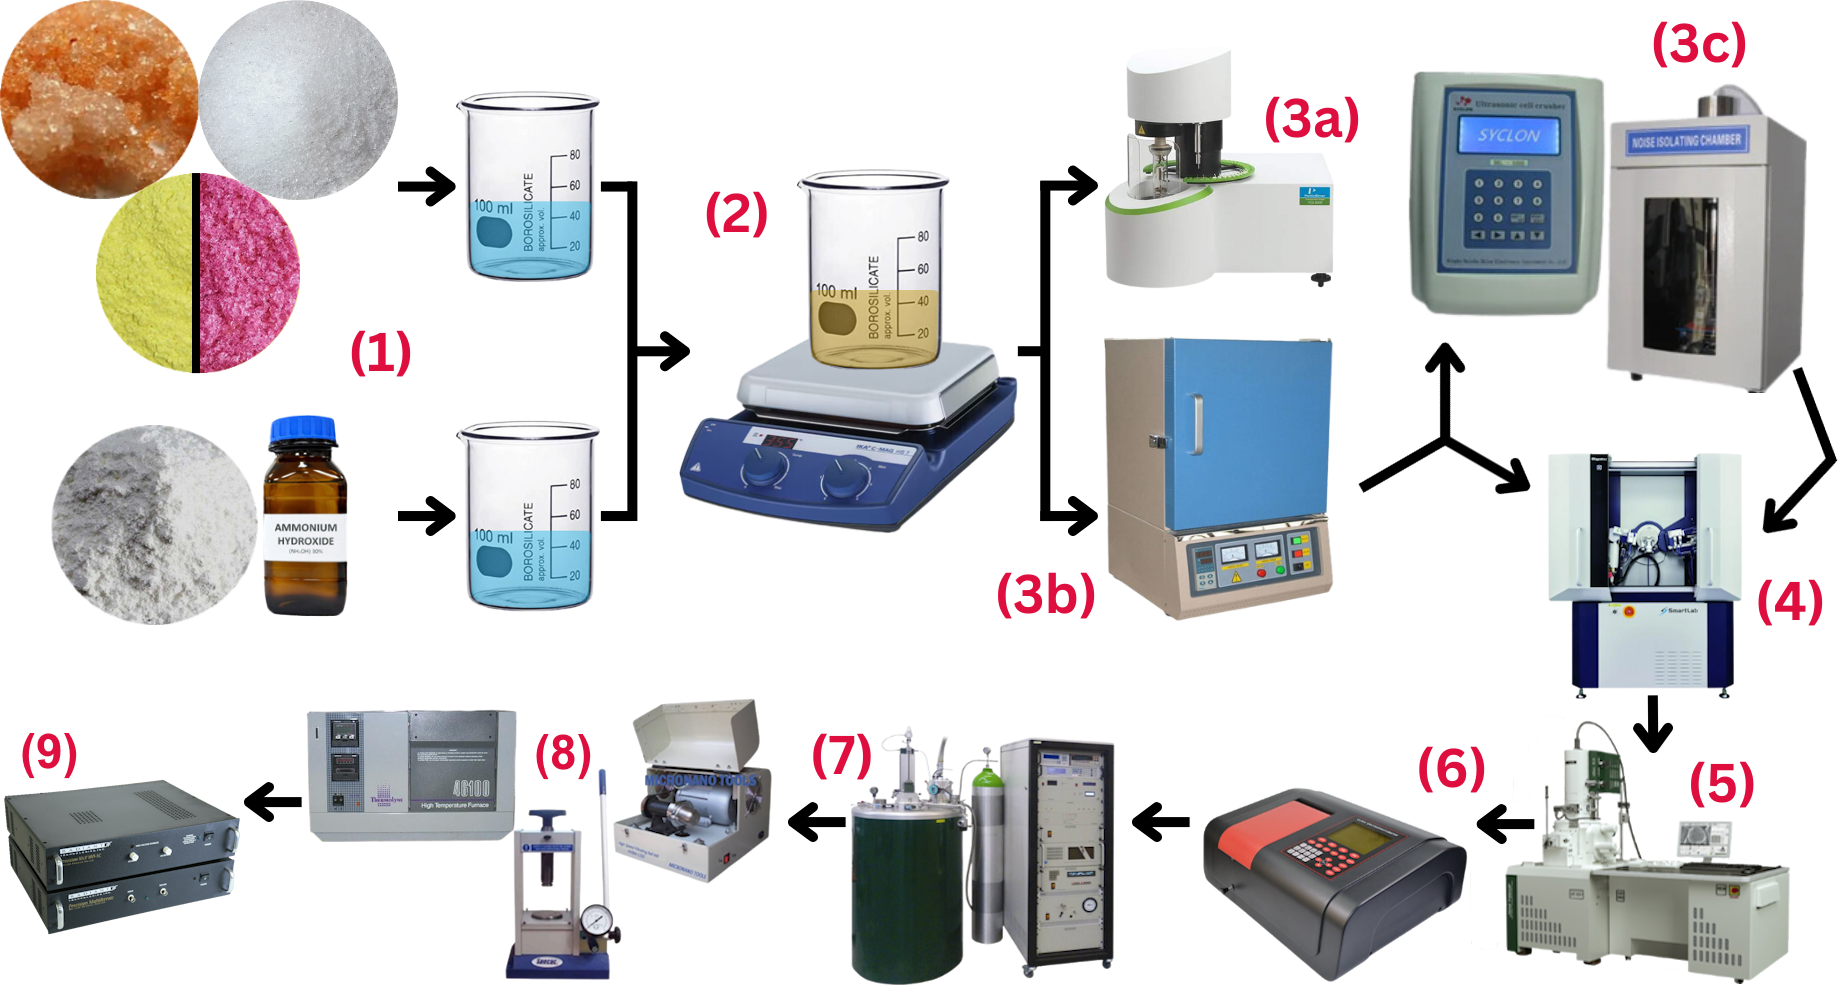
\includegraphics[width=0.75\textwidth]{fig/2.png}
    \caption{Diagrama de flujo del proceso de síntesis y caracterización seguido.}
    \label{fig:diagflujosint}
\end{figure}
\section{Síntesis}
En el caso del \neod{} se utilizaron los reactivos \ce{Fe(NO3)3 9H2O} (Nitrato de Hierro (III)) (Meyer, 98\%), \ce{Nd(NO3)3 6H2O} (Nitrato de Neodimio (III)) (Sigma-Aldrich, 99.9\%), \ce{C6H8O7} (ácido cítrico) (Meyer, 99.5\%) y \ce{C10H16N2O8} (EDTA) (Meyer, 99.4\%), además de \ce{NH4OH} (Hidróxido de Amonio) (J. T. Baker 28.0-30.0\%), que se utiliza para disolver el EDTA en agua desionizada, además de neutralizar el pH de la mezcla. Por otro lado, para la síntesis del \sama{} se utilizaron los mismos reactivos a excepción del \ce{Nd(NO3)3 6H2O}, el cuál fue sustituido por \ce{Sm(NO3)3 6H2O} (Nitrato de Samario (III)) (Sigma-Aldrich, 99.999\%). Esto con el fin de obtener la siguiente reacción:
\begin{equation}
    \ce{Fe(NO3)3 + 9H2O + R(NO3)3 + 6H2O -> RFeO3 + CO2 + NO2 + ...}
    \label{eq:reaccion}
\end{equation}
Donde \ce{R=Nd, Sm}.

Mediante una relación estequiométrica, se obtuvieron las cantidades que se muestran en la Tabla \ref{tab:sintesisneod} por cada gramo de \ce{NdFeO3} sintetizado:
    \begin{table}[H]
        \centering
        \begin{tabular}{|c|c|}
        \hline
        Compuesto&Masa\\
        \hline
        \ce{Fe(NO3)3}&1.628g\\
        \ce{Nd(NO3)3}&1.7665g\\
        \ce{C6H8O7}&0.774g\\
        \ce{C10H16N2O8}&1.1775g\\
        \hline
    \end{tabular}
    \caption{Cantidad de cada compuesto necesaria para sintetizar 1g de \neod{}.}
    \label{tab:sintesisneod}
    \end{table}
Por su parte, la relación estequiométrica por cada gramo de \sama{} es la que se muestra en la Tabla \ref{tab:sintesissama}:
    \begin{table}[H]
        \centering
        \begin{tabular}{|c|c|}
        \hline
        Compuesto&Masa\\
        \hline
        \ce{Fe(NO3)3}&1.5875g\\
        \ce{Sm(NO3)3}&1.7465g\\
        \ce{C6H8O7}&0.755g\\
        \ce{C10H16N2O8}&1.1485g\\
        \hline
    \end{tabular}
    \caption{Cantidad de cada compuesto necesaria para sintetizar 1g de \sama{}.}
    \label{tab:sintesissama}
    \end{table}
    En cada caso, los reactivos se mezclaron en dos vasos de precipitados con 20ml de agua desionizada cada uno, el EDTA y el hidróxido de amonio en un vaso y el resto de los compuestos en otro, como se observa en la figura \ref{fig:diagflujosint} (1), se calentó el vaso que contenía EDTA a alrededor de 60\gradoC{} mientras éste se disolvía y posteriormente se añadió el contenido del otro vaso de precipitados. Una vez hecho ésto, se comprobó que se tuviera un pH neutro y se subió la temperatura gradualmente hasta que la mezcla alcanzó alrededor de 80\gradoC{}, lo cual se ilustra en la figura \ref{fig:diagflujosint} (2), ésto con el fin de que se combustionara. Finalmente, el producto de esta combustión se molió haciendo uso de un mortero. 
    
    Se separó una muestra por cada tierra rara para realizar un análisis termogravimétrico, mostrado en la figura \ref{fig:diagflujosint} (3a), del cual se hablará en una sección posterior.

    El resto de muestras se calcinó por 12 horas, indicado en la figura \ref{fig:diagflujosint} (3b) haciendo uso de un horno BR-12N-3 de la marca Brother Furnace, con una rampa de calentamiento de 10\gradoC{}/min al subir la temperatura y 720 minutos constante en la temperatura objetivo. En cada muestra se utilizó una temperatura de calcinación distinta, ésta fue variada con intervalos de 100\gradoC{} entre cada muestra, empezando en 500\gradoC{} (600\gradoC{} en el caso del \sama{}) y terminando en 1000\gradoC{}.
\subsection{Sonicación}
    Además de esto, se sintetizaron dos muestras adicionales de \neod{} calcinadas a 600\gradoC{} y \sama{} calcinadas a 700\gradoC{}, a éstas se les sometió a un proceso de sonicación a 292W con una punta ultrasónica modelo UH-650W de la marca HNZXIB Lab, una por 2h y otra por 4h, lo cual se muestra en la figura \ref{fig:diagflujosint} (3c).

    Esta técnica funciona a través de un generador electrónico que transforma una entrada de corriente alterna a una señal de 20kHz, la cual controla un convertidor piezoeléctrico para generar vibraciones mecánicas de alta frecuencia, las cuales son transmitidas a una punta ultrasónica la cual se sumerge en una solución que consiste en la muestra a sonicar y agua destilada. Las vibraciones de la punta generan burbujas microscópicas, en un fenómeno conocido como cavitación. Éstas, al colapsar, liberan una gran cantidad de energía, la cual es suficiente para romper las partículas en suspensión \cite{sonicaciondef}.

    La potencia de sonicación está limitada por la punta utilizada, en este caso el fabricante indica que el máximo para la punta utilizada es el 45\% de la potencia máxima del equipo, lo que equivale a 292W \cite{manualpunta}.
\section{Caracterización}

\subsection{Análisis Termogravimétrico (TGA)}
Esta técnica de caracterización, cuyo equipo se observa en la figura \ref{fig:diagflujosint} (3a), y un diagrama de su estructura en la figura \ref{fig:diagTGA}, consiste en pesar continuamente una muestra mientras se calienta, la cuál se encuentra en una atmósfera de gas inerte. Muchos sólidos experimentan reacciones que producen subproductos gaseosos, estos subproductos gaseosos se eliminan y se registran los cambios en la masa restante de la muestra. Mediante éste es posible encontrar la temperatura a la que ocurren distintas transformaciones en la sustancia, sean estas reacciones químicas, o cambios físicos, como la cristalización.
\begin{figure}[H]
    \centering
    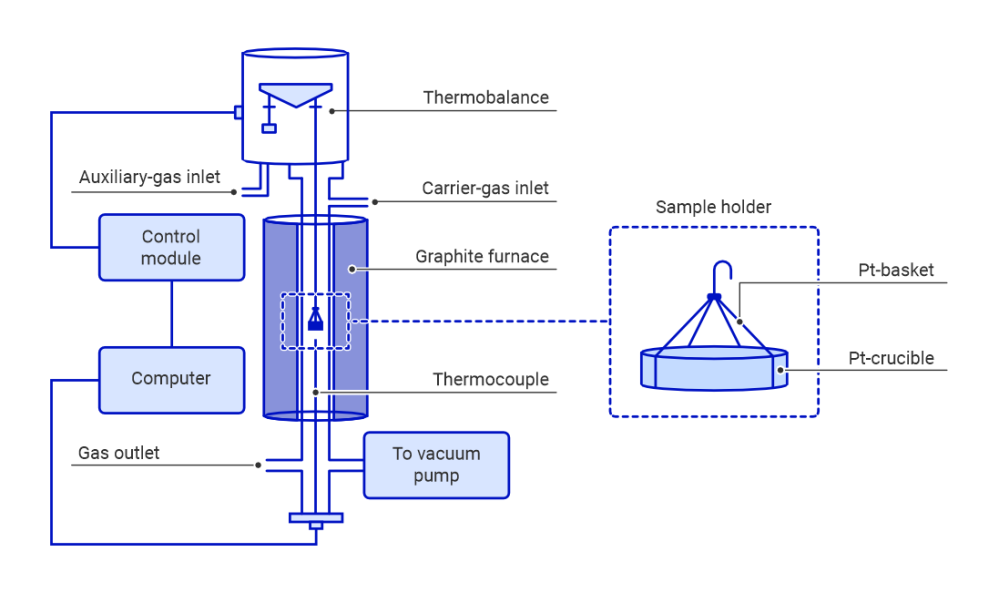
\includegraphics[width=0.7\textwidth]{fig/tgadiag.png}
    \caption{Diagrama de las partes que componen al equipo necesario para realizar un TGA. Adaptado de \cite{TGADIAG}.}
    \label{fig:diagTGA}
\end{figure}
Los procesos que se observan mediante esta técnica pueden ser endo o exotérmicos, debido a que tienen un efecto en el cambio de temperatura del material, sin embargo, dado que esta técnica no mide directamente la energía térmica de la muestra, no es posible diferenciar entre estos procesos sólo con los datos obtenidos mediante esta técnica \cite{TGA}.

Sin embargo, es posible inferir información sobre la posible temperatura a la que ocurre la cristalización al comparar los datos obtenidos con la temperatura de los cambios que se espera ocurran en la muestra. En este caso, se espera que haya una combustión de la fase orgánica y la evaporación del agua contenida en la muestra entre los 100 y 200\gradoC{}, mientras que la fase metálica es estable hasta temperaturas mucho más altas que las máximas alcanzadas por el equipo ($\approx1000$\gradoC{}), por lo que es posible asociar un proceso que ocurra a una temperatura mayor a 200\gradoC{} a la cristalización.

Se utilizó un \textit{detector}, el cual se configuró con una rampa de calor de $10$\gradoC{}$/$min que fue de 30\gradoC{} hasta 845\gradoC{}.
\subsection{Difracción de Rayos X (DRX)}
Esta técnica, cuyo equipo se puede observar en la figura \ref{fig:diagflujosint} (4) se basa en la interferencia constructiva que ocurre al irradiar una muestra cristalina con un haz de rayos X monocromados en ángulos que dependen de las fases que contenga la muestra. Funciona a través de un tubo de rayos catódicos que bombardea con electrones a un objetivo, los cuales, al tener la energía suficiente, desplazarán los electrones más internos de los átomos del objetivo a niveles energéticos más altos, los cuales a su vez, al regresar al estado de menor energía liberan rayos X de una longitud de onda característica que depende el material objetivo utilizado, los cuales irradian la muestra que se quiere medir en un arreglo como el que se ilustra en la figura \ref{fig:diagDRX}, lo cual brinda información sobre las fases contenidas en la muestra, como se explicará en las siguientes secciones \cite{dutrowxrd}.
\begin{figure}[H]
    \centering
    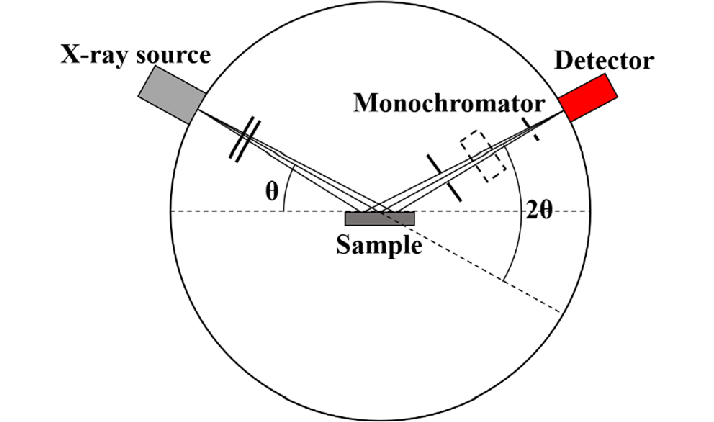
\includegraphics[width=0.6\textwidth]{fig/DRXdiag.png}
    \caption{Arreglo experimental utilizado para la obtención de espectros de difracción de rayos X. Adaptado de \cite{Jung2023}}
    \label{fig:diagDRX}
\end{figure}

Se utilizó un \textit{detector} para las muestras en polvo, y un  difractómetro \textit{Rigaku Ultima IV} para las muestras sinterizadas, ambos con fuentes de Cobre ($K_\alpha=1.54$\r{A}), la medición se realizó con $2\theta\in(20^\circ,80^\circ)$.
\subsubsection{Estructura Cristalina}
Los átomos y moléculas que conforman la mayoría de sólidos, como el cuarzo, la sal, los metales o los óxidos, se encuentran en un arreglo periódico regular, ésto se conoce como cristalinidad, y a la estructura periódica como estructura cristalina.

Pensando en cada átomo pertenecientes a un cristal como un punto, podemos expresar un cristal en 3 dimensiones como el conjunto de puntos que cumplen:
\begin{equation}
    \pmb{R}=\sum_{i=1}^{3} n_i\pmb{a_i}  
    \label{eq:estrcrist}
\end{equation}
Donde $\pmb{a_i}$ son vectores no colineales que representan cada dirección del cristal, cuyo tamaño es la separación entre átomos en esa dirección, además, $0\leq n_i<N_i$ es un número entero, donde $N_i$ es el tamaño máximo del cristal en esa dirección.

La estructura que forma esta construcción, incluyendo los ángulos entre cada vector $\pmb{a_i}$, se conoce como red de Bravais. Existen sólo 14 posibles redes, como se puede ver en la figura \ref{fig:bravais} las cuáles pueden definirse a través de su celda unitaria, que representa la unidad mínima del cristal que, al repetirse periódicamente en todas direcciones, genera el cristal entero \cite{Ashcroft1976}.
\begin{figure}[H]
    \centering
    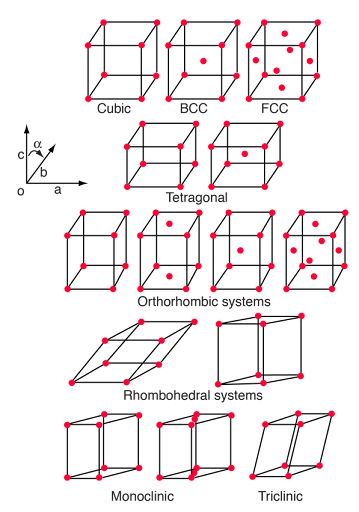
\includegraphics[width=0.75\textwidth]{fig/bravais.png}
    \caption{Redes de Bravais. Adaptado de \cite{ScienceFacts2024}.}
    \label{fig:bravais}
\end{figure}
Es posible expresar la orientación de cualquier plano que corte la estructura cristalina a través de los índices de Miller, éstos se obtienen a partir de las distancias entre el origen y los puntos en los que el plano intersecta a los ejes, expresado como fracciones de la distancia entre átomos en ese eje. Si se tomaran directamente estas distancias, no se podría tratar directamente con planos perpendiculares a los generados por los ejes, debido a que la intersección entre estos ocurre en el $\infty$, por esta razón, los índices de Miller se definen a través del recíproco de estas distancias, tomando 0 como recíproco de $\infty$, dando como resultado 3 números $h$, $k$, $l$, que se expresan como $(hkl)$, si alguno fuese negativo se escribe con una barra encima, $\left(\bar{h}kl\right)$. Finalmente, los 3 números obtenidos se multiplican por una constante para obtener el conjunto de enteros más pequeños generable con la menor cantidad de números negativos para ese trío de números \cite{Cullity2014}.
\paragraph{Ley de Bragg}
Si se tienen dos ondas que inicialmente están en fase, y se hace que una de éstas tome un camino más largo que la otra, para posteriormente reunirlas, éstas tendrán ahora una diferencia de fase igual a la diferencia en longitud de ambos caminos. Ésto es relevante para la derivación de la ley de Bragg debido a la estructura periódica del cristal, debido a la forma en la que éstos difractan rayos X.

La figura \ref{fig:braggdiag} muestra la sección de un cristal, cuyos átomos se encuentran ordenados en los planos paralelos $A$, $B$, ..., los cuales están separados por una distancia $d'$. A éste cristal se le irradia con una fuente de rayos X monocromática de longitud de onda $\lambda$ en un ángulo $\theta$. Considerando dos rayos cualesquiera que golpeen al cristal, éstos al ser dispersados estarán en fase, y por lo tanto interferirán sólo de manera constructiva, si y sólo si la diferencia entre la longitud de sus caminos es de $n\lambda$, lo cuál se conoce como difracción.
\begin{figure}[H]
    \centering
    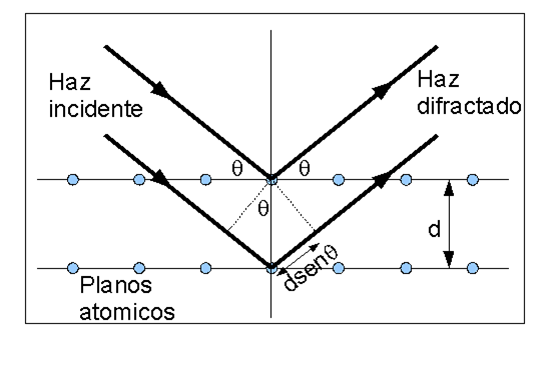
\includegraphics[width=0.7\textwidth]{fig/braggdiag.png}
    \caption{Difracción de rayos X por un cristal. Adaptado de \cite{Cullity2014}.}
    \label{fig:braggdiag}
\end{figure}
En la figura \ref{fig:braggdiag}, la recta $X$ representa el emisor de fotones, mientras que la recta $Y$ el detector de éstos.

Se tienen en esta figura dos rayos, uno compuesto por los segmentos $\overline{XK}$ (azul) y $\overline{KY}$ (naranja), y otro compuesto por los segmentos $\overline{XN}$ (rojo), $\overline{MN}$ (rosa), $\overline{LN}$ (amarillo) y $\overline{NY}$ (verde), como se muestra en la figura \ref{fig:braggdiag}.

Tomando en cuenta que los segmentos $\overline{XK}$ y $\overline{XN}$ son iguales, lo cual también ocurre para los segmentos $\overline{NY}$ y $\overline{KY}$, la diferencia en la distancia recorrida por ambos rayos se puede expresar como:
\begin{equation}
    \begin{split}
        (\overline{XM}+\overline{ML}+\overline{LN}+\overline{NY})-(\overline{XK}+\overline{KY})&=(\overline{XK}+\overline{ML}+\overline{LN}+\overline{KY})+(\overline{XK}+\overline{KY})\\
        &=\overline{ML}+\overline{LN}=2d'\sin{\theta}
    \end{split}
    \label{eq:rayosbragg}
\end{equation}

Es decir, éstos forman un rayo difractado si y sólo si:
\begin{equation}
    n\lambda=2d'\sin{\theta}
    \label{eq:leydebragg}
\end{equation}
Esta ecuación se denomina ley de Bragg \cite{Cullity2014}.
\subsubsection{Refinamiento Rietveld}
El método de Rietveld es una técnica de refinamiento que permite estudiar los patrones de difracción generados por rayos X de manera cuantitativa. Esta técnica permite encontrar información sobre la composición de la muestra, las fases cristalinas existentes en ésta y la posible presencia de contaminantes que posean una fase cristalina.

Consiste en utilizar el método de mínimos cuadrados para ajustar un modelo teórico a un patrón experimental de rayos X. Para este modelo se deben tomar en cuenta factores tales como aspectos estructurales (geometría de la celda unitaria, posiciones atómicas, vibraciones térmicas), microestructurales (mezcla de fases, concentración, deformaciones) e instrumentales (anchura de las rejillas utilizadas, tamaño de la muestra irradiada) \cite{Rietveld}. La función a minimizar se define entonces como
\begin{equation}
    S_y=\sum_i W_i\left(y_{i}-y_{i,c}\right)^2
    \label{eq:minimcuad}
\end{equation}
Donde $y_{i}$, $y_{i,c}$ son las intensidades observadas y calculadas respectivamente y $W_i$ es el peso dado a cada una de éstas, usualmente $1/y_i$ \cite{Fuentes2004}.

Por su parte, es posible expresar $y_{i,c}$ de la siguiente forma \cite{Rietveld}:
\begin{equation}
    y_{i,c}=\sum_j y_{i,j}=\sum_{j}S_j\sum_{k}L_{k,j}F^2_{k,j}\phi_{k,j}\left(2\theta_i-2\theta_{k,j}\right)P_{k,j}A+y_{b,i}
    \label{eq:intcalculada}
\end{equation}
Donde:
\begin{itemize}
    \item $y_{i,c}$ es la intensidad calculada en el punto $i$ del patrón de difracción.
    \item $y_{i,j}$ es la intensidad en el punto $i$ del patrón de difracción debido a la fase $j$.
    \item $S_j$ es el factor de escala correspondiente a la fase $j$.
    \item $k$ representa al pico de difracción k-ésimo del patrón de difracción.
    \item $L_{k,j}$ representa los factores de Lorentz, polarización y factor de multiplicidad.
    \item $F^2_{k,j}$es el factor de estructura de la fase $j$.
    \item $\phi_{k,j}(2\theta_i-2\theta_{k,j})$ es la función que describe el pico de difracción centrado en el ángulo $2\theta_{k,j}$ de la fase $j$. Ésta puede ser gaussiana, lorentziana o una combinación lineal de ambas.
    \item $P_{k,j}$ es la función que describe la orientación preferencial cuando los cristales de la fase $j$ no se encuentran en forma aleatoria.
    \item $A$ es un factor de absorción que depende del espesor de la muestra y la geometría del equipo de difracción.
    \item $y_{b,i}$ es la intensidad del fondo en el punto $2\theta_i$ del patrón de difracción.
\end{itemize} 
Para realizar éste análisis, se utilizó el programa \textit{MAUD - Materials Analysis Using Diffraction} \cite{MAUD}, el cual permite importar datos teóricos de cada una de las fases cristalinas, obtenidos de \cite{COD}, para calcular las intensidades teóricas utilizadas en el método Rietveld y utilizar éstas en conjunto con los datos experimentales en el refinamiento para minimizar $S_y$ (ecuación \ref{eq:intcalculada}) a través de los parámetros descritos anteriormente. Ésto dando como resultado gráficas como la que se muestra en la figura \ref{fig:picosrietveld}, además del porcentaje que representa cada fase en la muestra y la calidad del ajuste a través de los criterios que se discutirán en la sección \ref{sec:refinamiento}.
\begin{figure}[H]
    \centering
    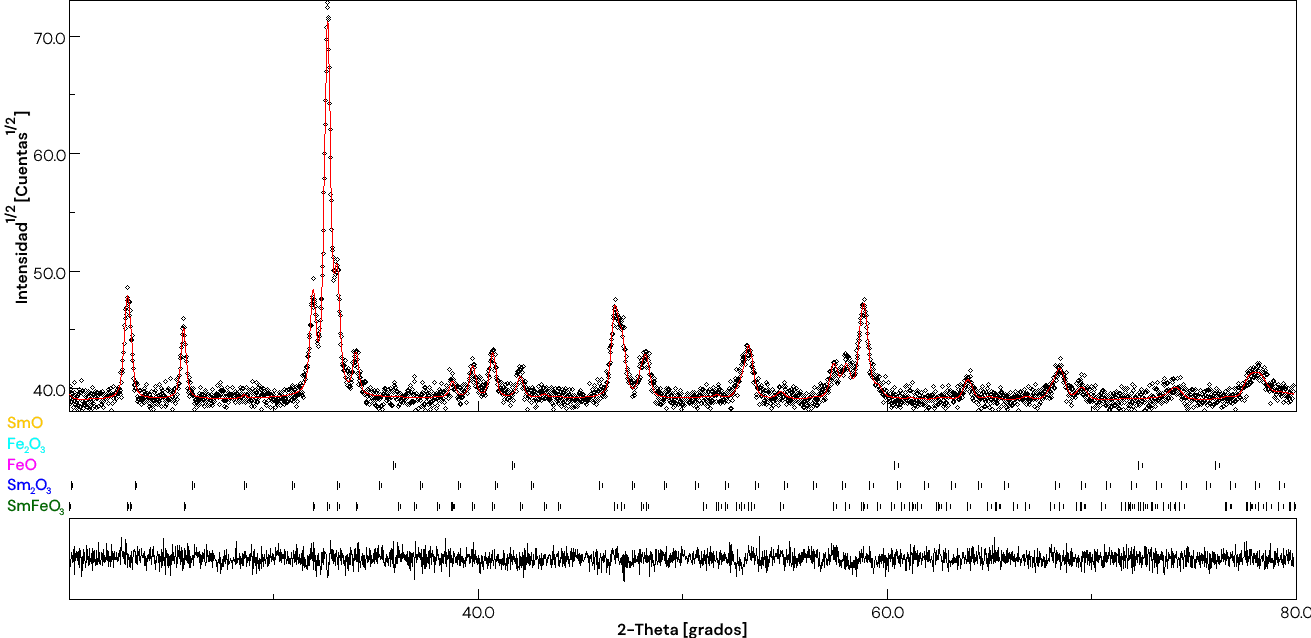
\includegraphics[width=0.7\textwidth]{fig/Rietveld.png}
    \caption{Modelado de picos de difracción utilizando \textit{MAUD}.}
    \label{fig:picosrietveld}
\end{figure}
\paragraph{Criterios de Refinamiento} \label{sec:refinamiento}
Existen diversos criterios de refinamiento cuyo valor permite conocer la calidad de éste. Los que se utilizaron para evaluar los resultados obtenidos son \cite{Rietveld}:
\begin{enumerate}[label=\textbf{\alph*)}]
    \item Residuo del patrón pesado ($R_{wp}$): Éste muestra el progreso del refinamiento, debido a que en el numerador contiene la función que se está minimizando (ecuación \ref{eq:intcalculada}). Se expresa de la siguiente manera:
    \begin{equation}
        R_{wp}=\left[\dfrac{\sum_i W_i\left(y_i-y_{i,c}\right)^2}{\sum_i W_i y_i^2}\right]^{1/2}
        \label{eq:patronpesado}
    \end{equation}
    \item Valor esperado ($R_{exp}$): Refleja la calidad de los datos obtenidos en la medición del patrón de difracción. Se expresa de la siguiente manera:
    \begin{equation}
        R_{exp}=\left[\dfrac{N-P}{\sum_i W_i y_i^2}\right]^{1/2}
        \label{eq:valoresperado}
    \end{equation}
    Donde $N$ es el número de datos observados y $P$ es el número de parámetros a refinar.
    \item Ajuste de bondad ($\chi^2$): Éste permite comparar el tamaño de los errores estadísticos ($R_{exp}$) con los errores producto del proceso de refinamiento ($R_{wp}$). Para que se considere que este método produjo un ajuste correcto, se busca que este criterio tenga un valor entre 1 y 1.3. Se expresa de la siguiente manera:
    \begin{equation}
        \chi^2=\dfrac{R_{wp}}{R_{exp}}
        \label{eq:ajustebondad}
    \end{equation}
\end{enumerate}
\subsection{Microscopía Electrónica de Barrido (SEM)}
Los microscopios electrónicos de barrido, de los cuales se muestra un diagrama en la figura \ref{fig:semdiag} y se ilustran en la figura \ref{fig:diagflujosint} (5), permiten lograr amplificaciones mucho mayores que las de un microscopio óptico a través del uso de electrones para generar la imagen.

Estos funcionan haciendo uso de una fuente de electrones, los cuales son acelerados con un potencial de 30kV y posteriormente son focalizados haciendo uso de lentes magnéticos. Se utilizan comúnmente tres de éstos, dos condensadores y un objetivo, siendo éste un determinante en la calidad de la imagen. Ésto produce un haz de electrones con un diámetro de entre 1 y 10nm.

Se generan campos magnéticos utilizando bobinas conectadas a generadores de ondas de escalera de $n$ y $m$ pasos, éstos cambian la dirección del haz, permitiendo escanear con éste una superficie rectangular dividida en $n\cdot m$ pixeles \cite{Egerton2005}.
\begin{figure}[H]
    \centering
    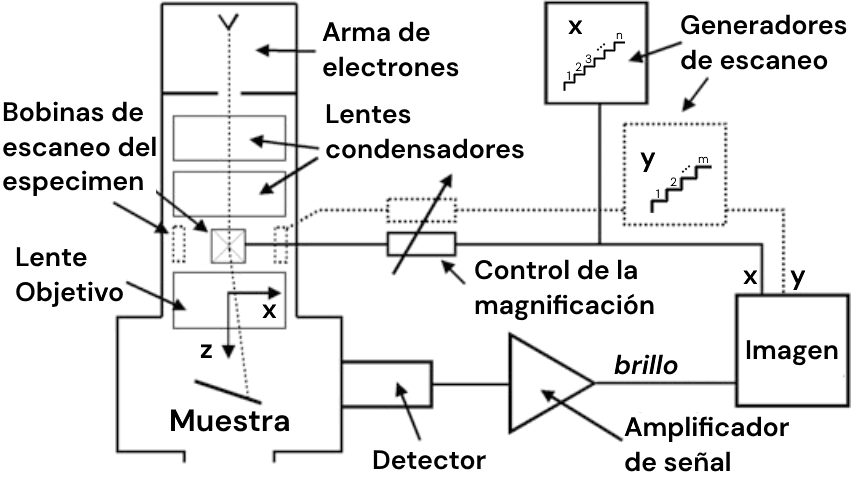
\includegraphics[width=0.7\textwidth]{fig/semdiag.png}
    \caption{Diagrama de un microscopio electrónico	de barrido. Adaptado de \cite{Egerton2005}.}
    \label{fig:semdiag}
\end{figure}
Se utilizó un microscopio \textit{JEOL JSM-7800F Schottky Field Emission Scanning Electron Microscope}, haciendo uso de un voltaje de 15kV, una corriente de 8 unidades arbitrarias y un vacío de $9.6\cdot10^{-5}$Pa.

Las muestras fueron preparadas colocando cada una en un portamuestras de aluminio cubierto con cinta de carbono, éstos materiales se utilizan debido a que no son magnéticos pero sí conducen la electricidad.

Estos portamuestras fueron colocados en una platina, la cual due ingresada a la cámara de vacío del microscopio, donde se realizó la medición. 

\subsubsection{Interacciones Electrón-Sólido}
Los electrones utilizados en un microscopio electrónico de barrido se conocen como electrones primarios cuando forman parte del haz generado. Una vez que éste entra a un sólido, cada electrón puede interactuar con los átomos presentes de diversas formas. Sin embargo, solamente tres son de interés, debido a que el resto no es medible por el microscopio electrónico. Éstas interacciones son las siguientes \cite{Egerton2005}:
\begin{itemize}
    \item  \textbf{Electrones Retrodispersados:} Al darse una colisión elástica, producto de la interacción electrostática electrón primario-núcleo, los electrones del haz se ven dispersados. La mayoría de estas deflexiones tienen un ángulo menor a 90\grado, lo cual implica que el haz permanece en el sólido, sin embargo, también pueden darse con un ángulo mayor, conservando la mayor parte de su energía inicial, esto haciendo muy probable que los electrones salgan del sólido, como se puede ver en la figura \ref{semtipos}a.
    \item \textbf{Electrones Secundarios:} En el caso de las colisiones inelásticas, producto de la interacción entre los electrones primarios y los electrones de valencia y conducción del sólido, cuando éstos colisionan, una pequeña parte de la energía se usa como energía potencial permitiendo al electrón salir de su orbital, conservando el resto de la energía perdida por el electrón primario como energía cinética. Aún así, la energía de los electrones producidos por este tipo de interacción es mucho menor a la anterior, permitiendo que escapen del sólido sólo aquellos más cercanos a la superficie. Ésto se ilustra en la figura \ref{semtipos}b.
    \item \textbf{Rayos X Característicos:} En éste caso, la colisión inelástica ocurre entre el electrón primario y un electrón de una capa interna del átomo, lo cual hace que éste pase brevemente a un estado de energía más alto y rápidamente decaiga de nuevo, liberando un fotón en el proceso. Este fotón estará en el rango de frecuencias de los rayos X, dependiendo el valor exacto de ésta solamente del número atómico Z del átomo, permitiendo conocer la composición química de la muestra. A ésta técnica se le conoce como Espectroscopía de Dispersión de Energía (EDS por sus siglas en inglés). Un ejemplo de esta interacción se muestra en la figura \ref{semtipos}c.
\end{itemize}
\begin{figure}[H]
    \centering
    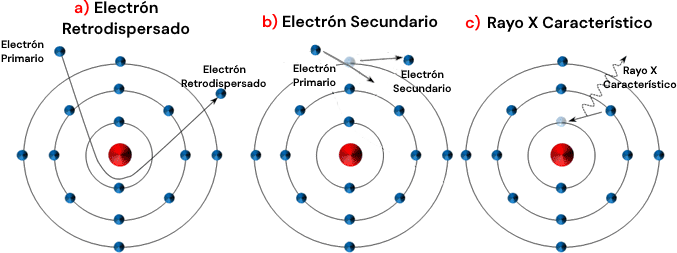
\includegraphics[width=0.7\textwidth]{fig/semtipos.png}
    \caption{Tipos de interacciones electrón-sólido en un microscopio electrónico de barrido. Adaptado de \cite{Jensen2022}.}
    \label{semtipos}
\end{figure}
En el caso de los EDS realizados, se utilizaron las mismas condiciones que en la obtención de imágenes, es decir, voltaje de 15kV, corriente en 8 unidades arbitrarias, presión de $9.6\cdot10^{-5}$Pa. Se registraron los rayos X emitidos por la muestra durante un minuto en cada medición.
\subsubsection{Análisis Estadístico del Tamaño de Partículas} \label{sec:analisisestadistico}
Las imágenes obtenidas a través de SEM fueron analizadas a través de ImageJ \cite{ImageJ}, éstas fueron procesadas definiendo la escala correcta en $\mu$m, en éste caso se tomaron las imágenes obtenidas en una amplificación de x500 debido a que éstas muestran de manera completa las partículas grandes mientras siguen siendo visibles las más pequeñas, como se puede ver en la figura \ref{fig:imgjcomp}a. Se prosiguió utilizando la función \textit{Threshold} para definir la posición de las partículas en la imagen, como se observa en la figura \ref{fig:imgjcomp}b, seguido de la función \textit{Analyze Particles} para seleccionarlas y medirlas, esto se puede ver en la figura \ref{fig:imgjcomp}c, lo cual dió como resultado una tabla que registra el diámetro de cada partícula detectada por el programa.
\begin{figure}[H]
    \centering
    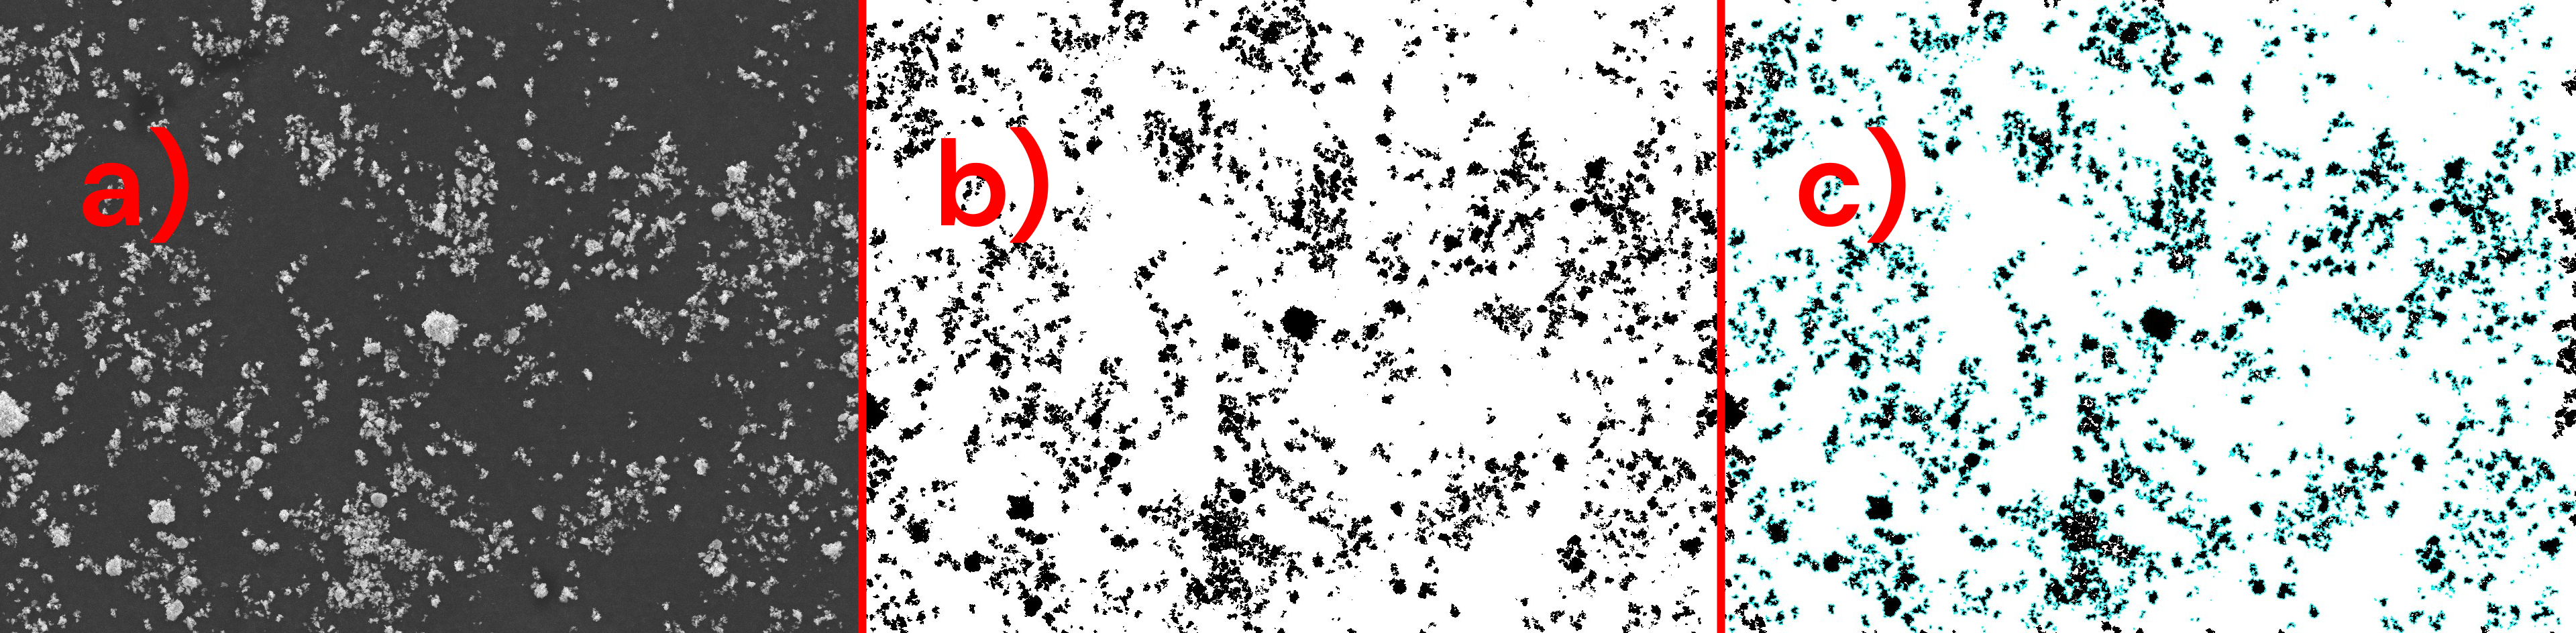
\includegraphics[width=0.7\textwidth]{fig/imagejcomp.png}
    \caption{Procesado de Imágenes con ImageJ.}
    \label{fig:imgjcomp}
\end{figure}
Para visualizar los datos obtenidos mediante este método, se empleó un histograma del diámetro de las partículas de cada muestra, como se observa en la figura \ref{fig:ejemplohist}.
\begin{figure}[H]
    \centering
    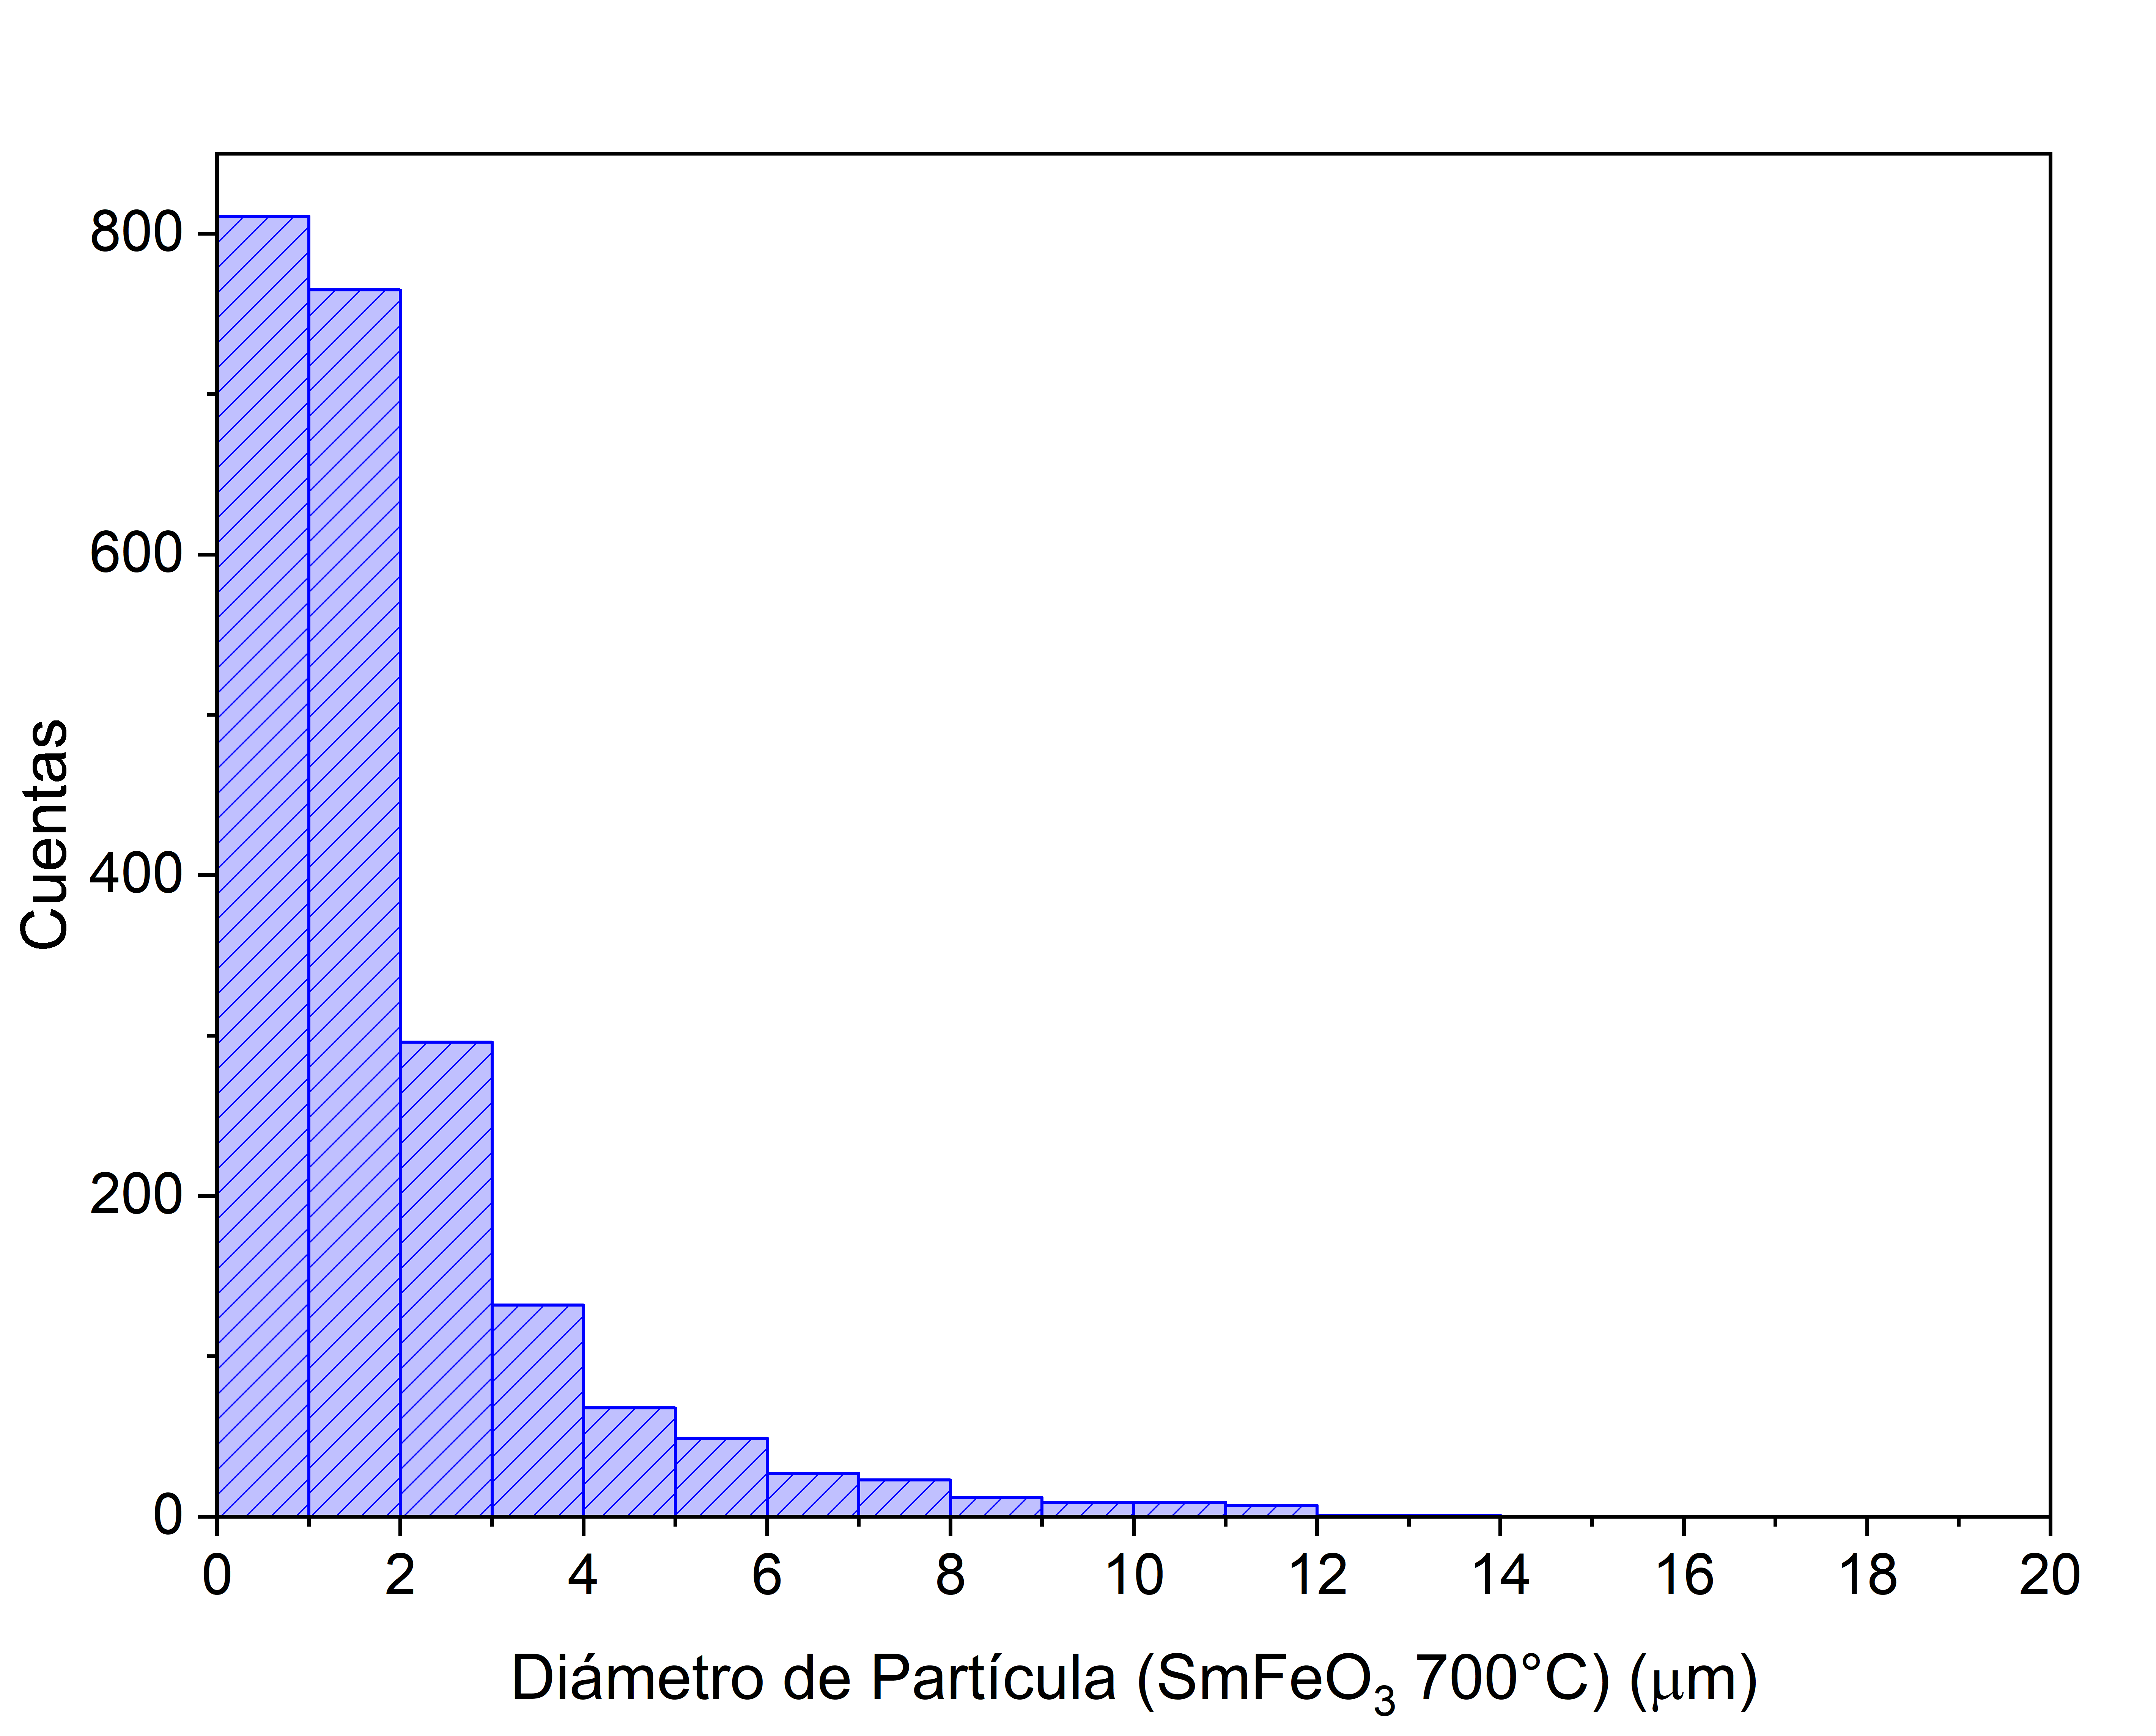
\includegraphics[width=0.7\textwidth]{fig/ejemplohist.png}
    \caption{Histograma de los datos obtenidos con ImageJ.}
    \label{fig:ejemplohist}
\end{figure}
Se obtuvo a partir de éste el porcentaje de partículas con un diámetro menor o igual a $1\mu$m. Éste se puede expresar de la siguiente manera:
\begin{equation}
    P=\dfrac{n}{N}\cdot100=p\cdot100
    \label{eq:porcentajeeq}
\end{equation}
Donde $n$ es el número de partículas con diámetro $\leq 1\mu$m, $N$ es el número total de partículas y $p=n/N$ es la proporción entre $n$ y $N$.

Suponiendo que cada medición tiene una probabilidad constante $a$ de estar en una determinada barra y que cada tamaño es independiente de los demás, la probabilidad $A$ de observar exactamente $n$ partículas de diámetro $\leq 1\mu$m es de:
\begin{equation}
    A(n)=\binom{N}{n}a^n(1-a)^{N-n}
    \label{eq:binomdist}
\end{equation}
Es decir, las barras siguen una distribución binomial, por lo que es posible utilizar la siguiente forma de la varianza \cite{Stephenson2005}:
\begin{equation}
    \text{Var}(n)=N\cdot p\cdot(1-p)
    \label{eq:varianza}
\end{equation}
Cuyas variables son las mismas que las descritas en la ecuación \ref{eq:porcentajeeq}. Finalmente, la raíz cuadrada de esta cantidad es la desviación estándar, la cual se expresa de la siguiente manera:
\begin{equation}
    \sigma_n=\sqrt{\text{Var}(n)}=\sqrt{N\cdot p\cdot(1-p)}
    \label{eq:desviacionsinescalar}
\end{equation}
Debido a que se busca encontrar la desviación estándar del porcentaje y no del número de partículas, se tiene lo siguiente:
\begin{equation}
    \begin{split}
        P=\dfrac{100}{N}\cdot n&\implies\sigma_P=\dfrac{100}{N}\cdot\sigma_n\\
        \iff \sigma_P=\dfrac{100}{N}\sqrt{N\cdot p\cdot(1-p)}&=\dfrac{100}{\sqrt{N}}\sqrt{p\cdot(1-p)}
    \end{split}
    \label{eq:desvest}
\end{equation}
Se puede utilizar el doble de la desviación estándar para asignar un valor de incertidumbre a ésta medición, debido a que ésta especifica cuantitativamente la precisión de una medida, ésto debido a que, para distribuciones binomiales, se tiene cerca del 95.45\% de los valores en el intervalo $(\bar{X}-2\sigma,\bar{X}+2\sigma)$, teniendo éste porcentaje en el límite en el que la distribución es normal \cite{bertaoda}.
\subsection{Espectroscopía UV-Vis}
Esta técnica, cuyo equipo se puede observar en la figura \ref{fig:diagflujosint} (6), mide la cantidad de luz UV o visible que es absorbida o transmitida a través de una muestra en comparación con una referencia o una muestra en blanco.

Cuando un fotón interactúa con la materia éste puede ser absorbido, lo cuál sólo ocurre si éste tiene la energía correcta para llevar un electrón de un estado a otro. Es por ésto que la absorción depende de la longitud de onda de la luz.
\begin{figure}[H]
    \centering
    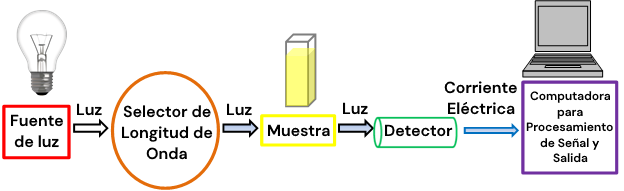
\includegraphics[width=0.7\textwidth]{fig/uvvisdiag.png}
    \caption{Diagrama de un espectrómetro UV-Vis. Adaptado de \cite{Tom2023}.}
    \label{fig:uvvisdiag}
\end{figure}
En la figura \ref{fig:uvvisdiag} se observa un diagrama simplificado del funcionamiento del equipo necesario para esta técnica. Comienza con una fuente de luz, comúnmente utilizándose dos lámparas, una de deuterio para la luz UV y una halógena para la luz visible. Ésto causa que el equipo cambie de lámpara alrededor de los 300-350nm, lo cual es necesario tomar en cuenta al analizar los datos.

Posteriormente, se hace pasar el haz de luz a través de monocromadores, además de filtros de absorción, de interferencia y de corte, ésto permite seleccionar un rango de frecuencias, el cual puede variarse y así analizar por separado las frecuencias que las lámparas emiten.

Después, el haz resultante se incide primero en una muestra en blanco para medir el fondo y restar éste de los datos que se obtengan, para luego incidir el haz sobre la muestra y registrar ya sea la absorbancia o reflectancia a través de detectores, los cuales funcionan haciendo uso de semiconductores o una capa fotoeléctrica, debido a que ambos generan una corriente proporcional a la intensidad de la luz incidente \cite{Tom2023}.

En el caso de las mediciones realizadas, se utilizó un espectrómetro modelo \textit{Macylab UV-1800CPC} en modo de absorción en precisión normal, utilizando luz de 200 a 800nm, con un paso de 0.2nm.
\subsubsection{Método Tauc}
Una de las propiedades ópticas más importantes en los semiconductores se conoce como brecha de energía prohibida o \textit{band gap}. Esta nos habla de la separación entre el estado más energético ocupado por los electrones del material (banda de valencia) y el estado siguiente (banda de conducción), este concepto se ilustra en la figura \ref{fig:diagbandgap}. El \textit{band gap} es la energía requerida para que un electrón pase de una banda a la otra \cite{Ashcroft1976}.
\begin{figure}[H]
    \centering
    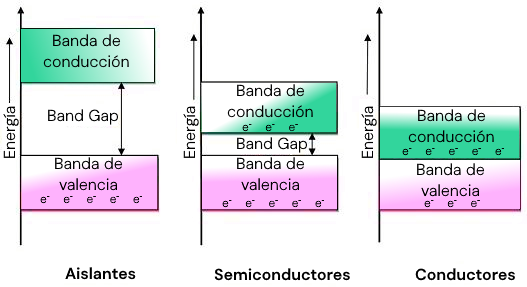
\includegraphics[width=0.7\textwidth]{fig/bandgapdiag.png}
    \caption{Diagrama del \textit{band gap} de distintos tipos de materiales. Adaptado de \cite{Ozan2020}.}
    \label{fig:diagbandgap}
\end{figure}
Sin embargo, los datos obtenidos a través de la espectroscopía UV-Vis no proporcionan esta propiedad directamente, sino que es necesario analizar los resultados a través del método Tauc.

Éste permite obtener el \textit{bang gap} del material estudiado partiendo de suponer que la absorbancia ($\alpha$) puede expresarse como:
\begin{equation}
    \begin{split}
        (\alpha\cdot h\nu)^{1/\gamma}=Bh\nu-E_g\\
        \iff (\alpha\cdot E_\nu)^{1/\gamma}=BE_\nu-E_g
    \end{split}
    \label{eq:taucalpha}
\end{equation}
Donde $h$ es la constante de Plank, $\nu$ es la frecuencia del fotón, $B$ es una constante, $\gamma=1/2, 2$ según se tenga un \textit{band gap} directo o indirecto respectivamente, $E_\nu$ es la energía de un fotón de frecuencia $\nu$ y $E_g$ es la energía del \textit{band gap} \cite{Makula2018}.

El espectrómetro, al medir absorbancia, permite conocer $\alpha$ respecto a $\nu$, por lo tanto basta con encontrar una zona de la gráfica de $(\alpha\cdot h\nu)^{1/\gamma}$ respecto a $h\nu$ que tenga un comportamiento lineal para así ajustar una recta por mínimos cuadrados y encontrar los valores que este ajuste arroje para $E_g$, como se puede observar en la figura \ref{fig:ejemplotauc}.
\begin{figure}[H]
    \centering
    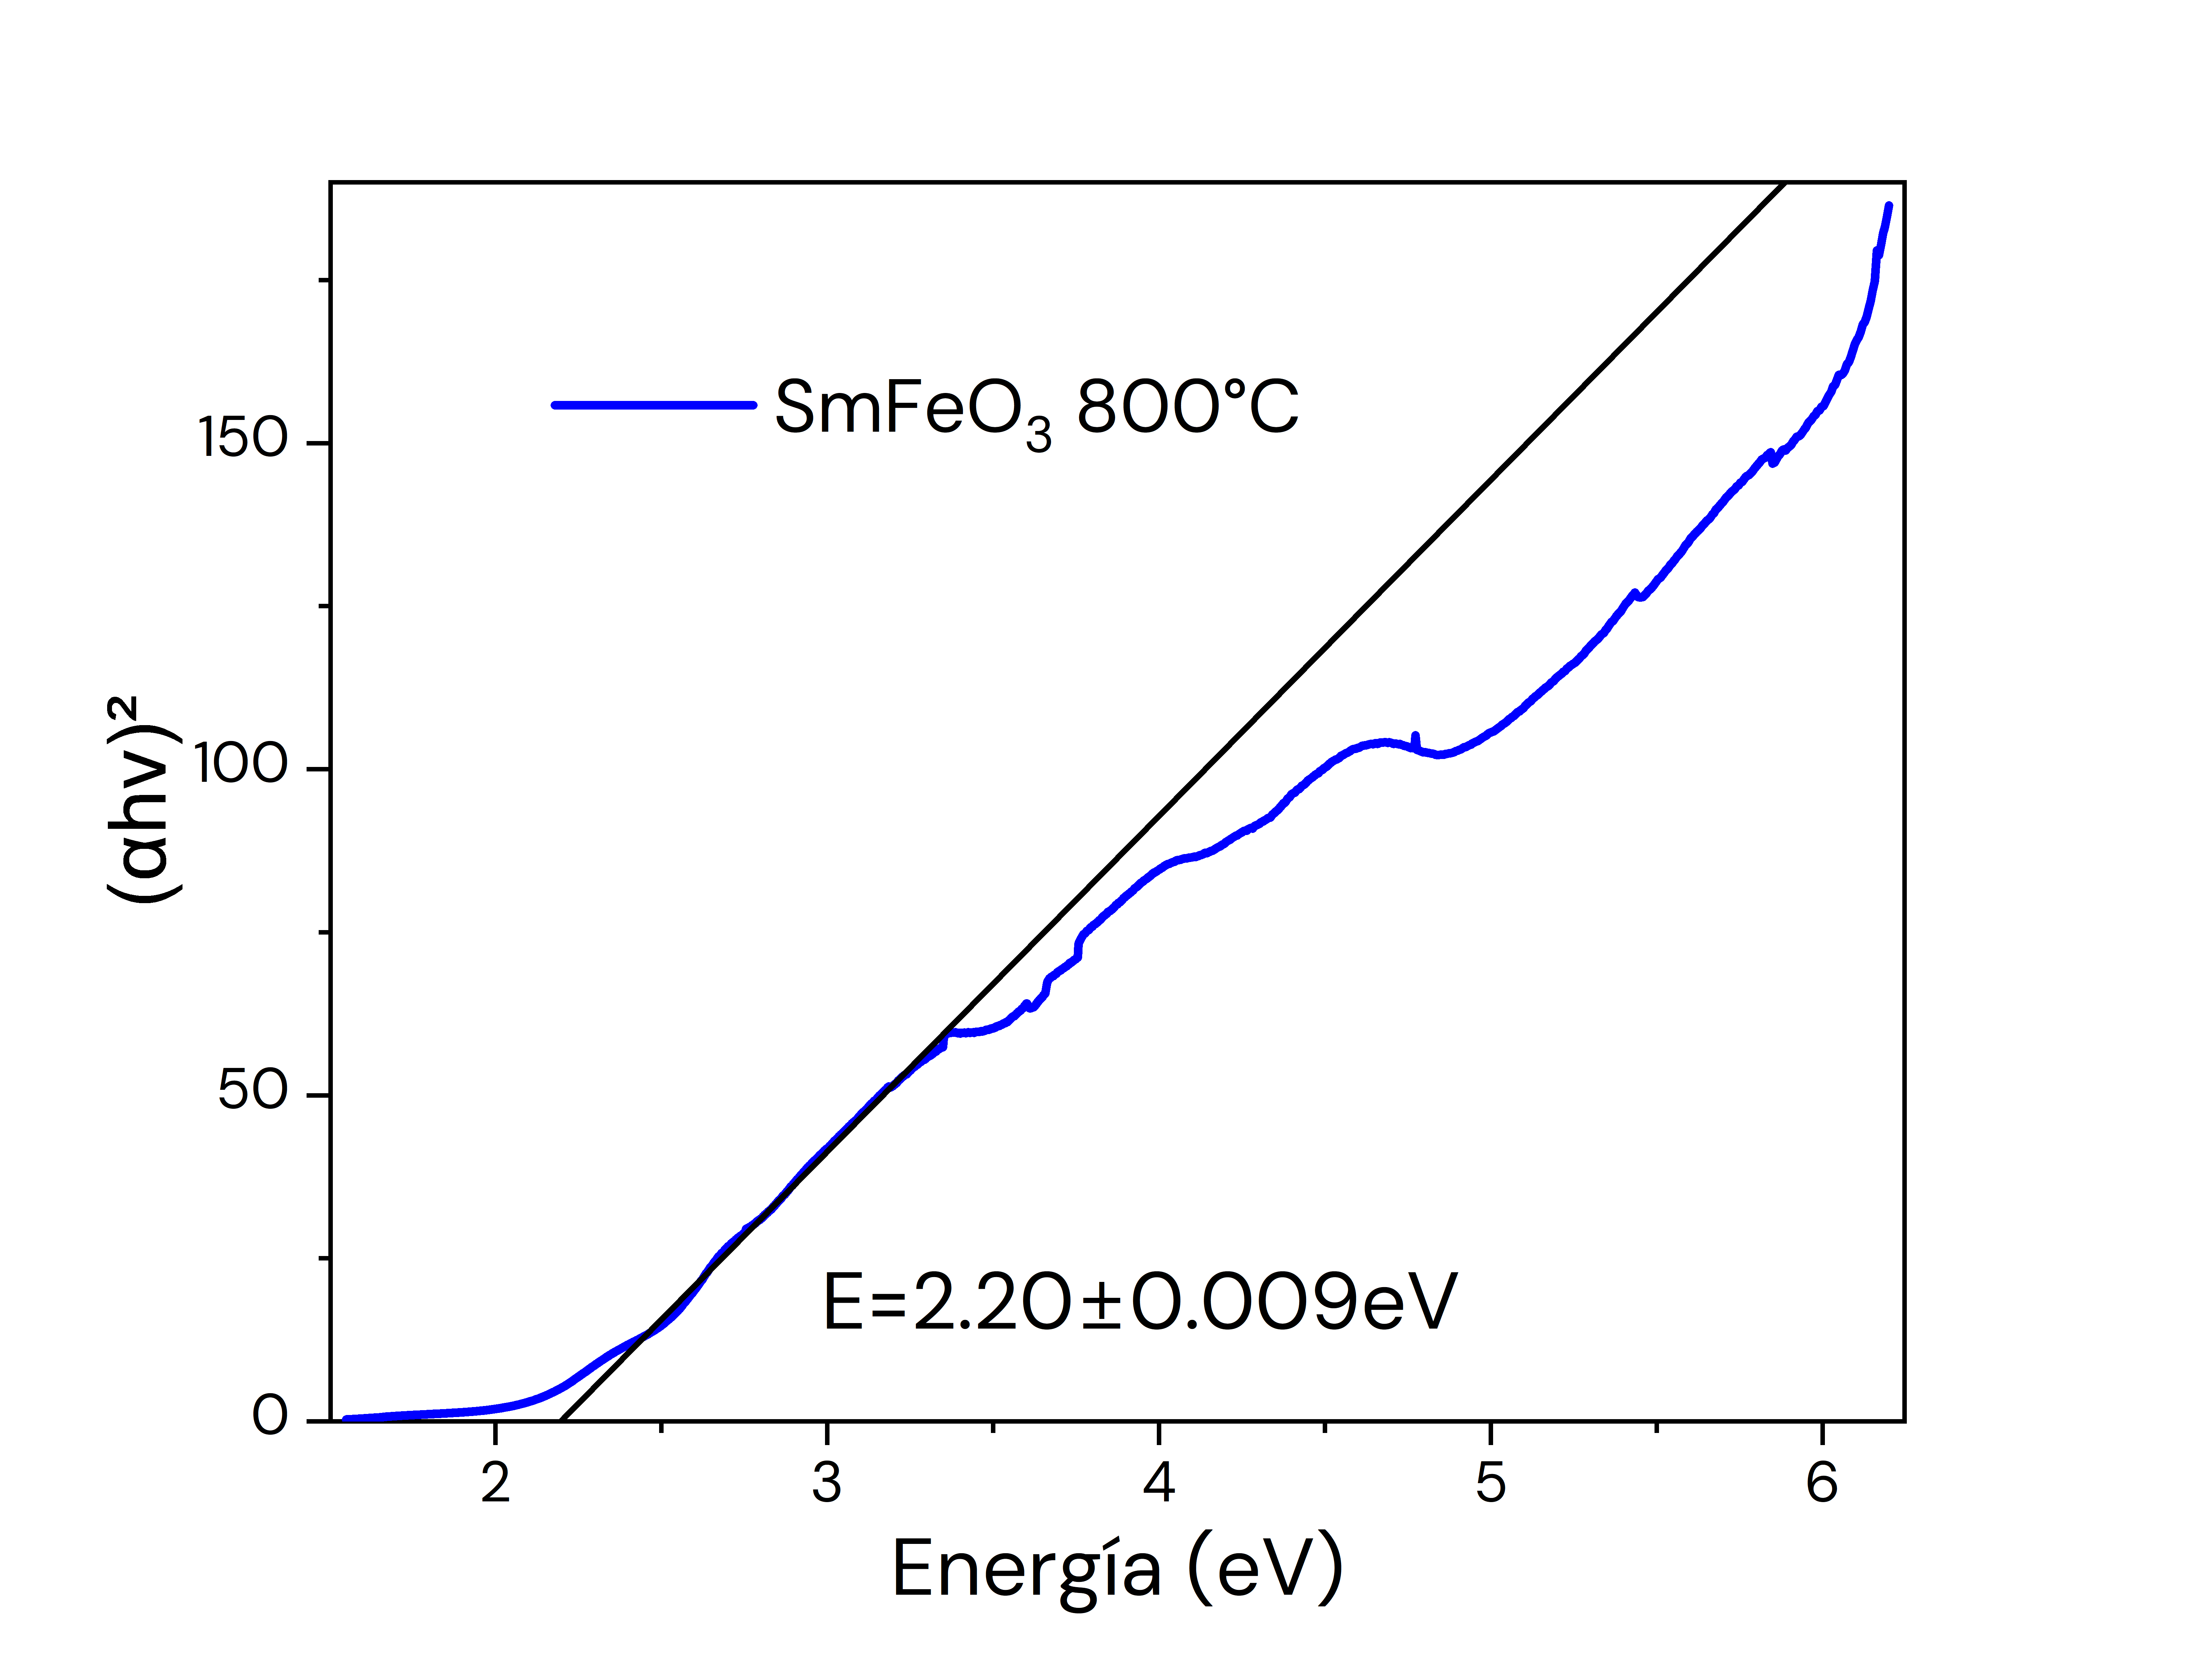
\includegraphics[width=0.6\textwidth]{fig/ejemplotauc.png}
    \caption{Aplicación del método Tauc para la muestra de \sama{} calcinada a 800\gradoC.}
    \label{fig:ejemplotauc}
\end{figure}
\subsection{Magnetometría}

\subsubsection{Dispositivo Superconductor de Interferencia Cuántica (SQUID)}

\paragraph{\textit{Zero Field Cooling} y \textit{Field Cooling}}

\paragraph{Mediciones Magnéticas Realizadas}

\subsection*{Mediciones Ferroeléctricas}

\subsubsection{Preparación de la Muestra}
Para conseguir medir la polarización contra la carga aplicada es necesario que la muestra sea un sólido. Para conseguir esto a partir de los polvos sintetizados se tuvo que realizar un proceso de molienda (sección \ref{sec:molienda}) y sinterización (sección \ref{sec:sinter}). Ésto se realizó con las ortoferritas calcinadas a temperatura más baja (600\gradoC{} para el \neod{} y 700\gradoC{} para el \sama{}), tanto a las muestras sin procesar como a las sonicadas por 4 horas a 292W.

\subsubsection{Molienda} \label{sec:molienda}
La molienda se realizó haciendo uso de un molino de bolas vibratorio de alta velocidad modelo \textit{HVBM-1200} de la marca \textit{MicroNanoTools}, que tiene una velocidad de 1200rpm \cite{Molino}.

Los molinos de bolas, en su forma más simple, consisten de un cilindro hueco, el cual se llena con la muestra a moler, las bolas a utilizar y opcionalmente un solvente o lubricante para limitar el calor generado.

Éste se monta en un motor que lo hace rotar, lo cual genera colisiones entre las bolas, el material y las paredes debido a la fuerza centrífuga, lo cual tiene como resultado el molido del material, lo que se ilustra en la figura \ref{fig:molinodiag} \cite{Baheti2012}.
\begin{figure}[H]
    \centering
    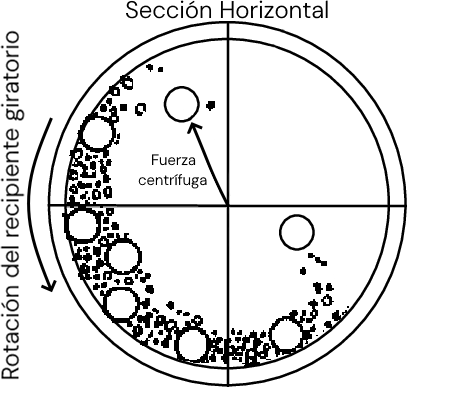
\includegraphics[width=0.4\textwidth]{fig/molinodiag.png}
    \caption{Diagrama de un molino de bolas. Adaptado de \cite{Baheti2012}.}
    \label{fig:molinodiag}
\end{figure}
Se colocaron 0.6g de la muestra a moler dentro de un reactor de Circonio con bolas del mismo material, con un diámetro de alrededor de 1cm, además de 30ml de isopropanol. Posteriormente se montó el reactor en un soporte de acero inoxidable y finalmente se aseguró en el molino, el cual se hizo funcionar por 20 minutos para cada muestra.

\subsubsection{Sinterización} \label{sec:sinter}
La sinterización es un tratamiento térmico de polvos metálicos o cerámicos en objetos sólidos a través de procesos de transporte de masa a nivel atómico, haciendo uso de presión y temperatura, sin que esta última llegue a la temperatura de fusión del material \cite{Banerjee2019}.

Un sólido debe tener una energía mayor en su superficie que en el resto del material pues la fuerza que la mantiene unida es menor. Esta energía libre de superficie ($G_s$) se describe a través de la energía libre de Gibbs $G$ y la tensión superficial $\gamma$ en una superficie $A$ de la siguiente manera:
\begin{equation}
    \gamma=\left(\dfrac{\partial G}{\partial A}\right)_{T,P,n}\\
    G_s=\sum_{i=1}^{m} n_i \mu_i + \gamma A
    \label{eq:energiasuperficie}
\end{equation}
Donde $n_i$ es la cantidad de moles de la sustancia $i$-ésima y $\mu_i$ es su potencial químico. Debido a que, al aumentar la superficie, $n_i$ es creciente para cualquier $i$, y debe ser estrictamente creciente para al menos una $i$, para alguna función $N(A)$ estrictamente creciente podemos escribir
\begin{equation}
    \sum_{i=1}^{m} n_i \mu_i = N(A)\\
    G_s(A)=N(A)+\gamma A
    \label{eq:energiasuperficiedepA}
\end{equation}
Donde $G_s(A)$ es estrictamente creciente. Debido a que ambos términos que componen a $G_s$ dependen de

Este proceso funciona a través de la difusión de los átomos en las fronteras entre granos, uniéndolos en el proceso, esto debido a la energía aplicada en forma de presión y calor, la cual provoca un reordenamiento de los cristales a una configuración de menor energía libre en su superficie, es decir, se eliminan las fronteras y las porosidades, como se muestra en la figura \ref{fig:sintdiag} \cite{Ou2014}.
\begin{figure}[H]
    \centering
    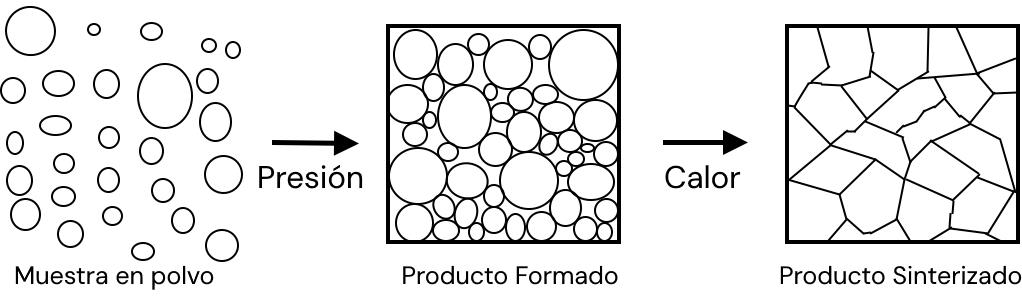
\includegraphics[width=0.8\textwidth]{fig/sintdiag.jpg}
    \caption{Diagrama del proceso de sinterización. Adaptado de \cite{Ou2014}.}
    \label{fig:sintdiag}
\end{figure}

Los resultados de este proceso dependen de la temperatura, presión aplicada, tiempo de sinterización e incluso de la presión atmosférica. En este trabajo se tomaron como condiciones de sinterización una presión de 5t aplicada por 15 minutos, realizado con una prensa hidráulica manual de 15t de marca \textit{SPECAC}, y una temperatura de 1000\gradoC{} aplicada por 2 horas, haciendo uso de un horno (\textit{nombre}) \cite{Aparnadevi2016}.

\subsubsection{Mediciones de Polarización}
Es posible obtener la polarización debido a que la carga ($Q$) en la muestra puede expresarse como:
\begin{equation}
    Q=\int_{t_1}^{t_2}I(t)\text{d}t
    \label{eq:cargaintensidad}
\end{equation}
Donde $I$ es la corriente que se hace pasar a través de la muestra en el tiempo $t$.

Con esto, podemos expresar el desplazamiento dieléctrico ($D$) como:
\begin{equation}
    D(t)=\dfrac{Q}{A}
    \label{eq:despdielec}
\end{equation}
Donde $A$ es el área superficial de la muestra.
\begin{equation}
    P(t)=D(t)-\epsilon_0E(t)
    \label{eq:polarizacionec}
\end{equation}
Finalmente, debido a que $E$ es una función de $t$ cuyo valor se controla a través del dispositivo, es posible graficar $P(E)$, lo cual es la medición buscada \cite{Stewart1999}.
\end{document}